%!TEX root = ./proposta3.tex


Uma arquitetura em \emph{cloud} envolve a comunicação entre inúmeros componentes através de APIs (\emph{Application Programing Interface}) de serviços web. Os usuários desta arquitetura não sabem e não precisam saber sobre a localização de seus dados ou as aplicações que desejem utilizar, porém precisam aceitar e dependem  dos níveis de segurança vigentes, que são tópicos preocupantes para os administradores.
A segurança em \emph{cloud} compreende as áreas de segurança de dados e da rede, segundo \cite{Dhage:2011:IDS:1980022.1980076}:  

Enquanto um ataque em dados afeta um número restrito de usuários, um ataque na rede pode comprometer diversos usuários simultaneamente. Como ataques de DDos em uma \emph{cloud} compreendem um ataque à segurança em rede, eles são de importância crítica.  
%Um dos mais importantes fatores para detectar ataques de DDoS é encontrar a correlação entre diferentes fluxos para um mesmo destino.
%
Com a nova infraestrutura de recursos criada pelas \emph{clouds}, existe a possibilidade de se mover fisicamente uma aplicação para outro endereço quando ela é atacada por DDoS. Com isso, pode se garantir tolerância à falhas e conservação de recursos despendidos, pois este novo endereço só será conhecido por solicitantes legítimos.

Este trabalho propõe uma arquitetura para mitigar ataques de DDoS em \emph{clouds} de forma autônoma e independente. As diferenças desta para outras propostas se concentram na independência da aplicação hospedada, em prover acurácia na filtragem de tráfego legítimo, por não onerar financeiramente o uso dos recursos, e por minimizar os problemas causados pelo ataque sem intervenção humana.
%
A arquitetura proposta poderá ser utilizada por qualquer aplicação web hospedada em uma \emph{cloud} que, ao sofrer indícios de um ataque DDoS, filtra o tráfego legítimo e encaminha apenas este para uma nova instância da mesma aplicação. 

%
\begin{figure}[h!]
\centering
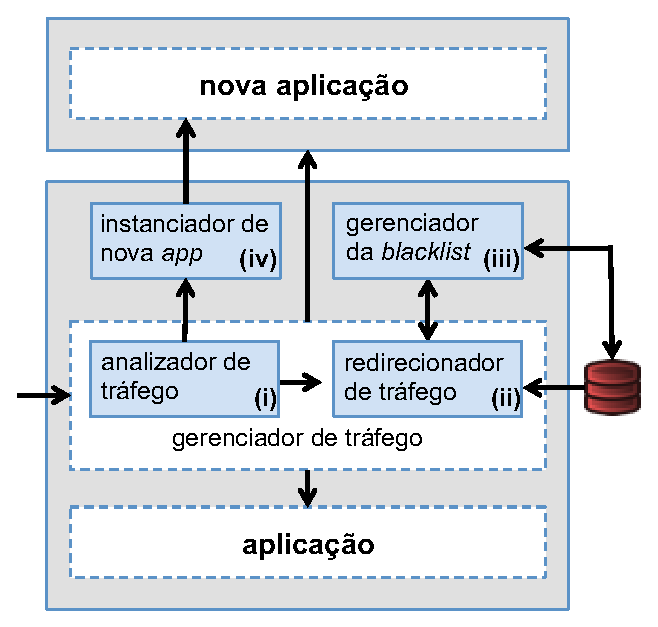
\includegraphics[width=0.55\textwidth]{images/arq.eps}
\caption{Ilustração da proposta de arquitetura para mitigação de ataques DDoS}
\label{fig:arq}
\end{figure}

\begin{figure}[h!]
\centering
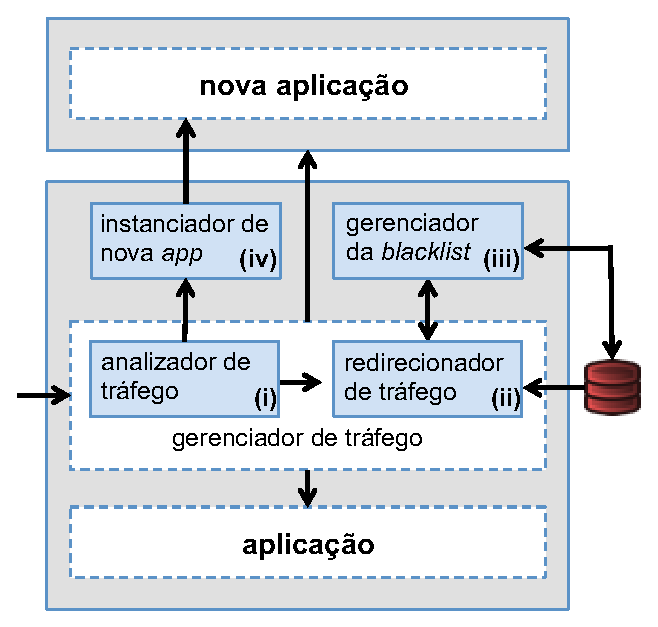
\includegraphics[width=0.55\textwidth]{images/arq.eps}
\caption{Ilustração da proposta de arquitetura para mitigação de ataques DDoS}
\label{fig:arq}
\end{figure}

Esta arquitetura, ilustrada na Figura \ref{fig:arq}, é composta por um módulo geral chamado de Gerenciador de Tráfego (GT), que não se comunica diretamente com a aplicação. Vale ressaltar que a instância do banco de dados é exterior às demais instâncias da \emph{cloud}, pelo fato de que este banco de dados também está nas nuvens, e pode ser acessado de qualquer outra instância \emph{cloud}. As operações realizadas pelo módulo GT são divididas em quatro submódulos:
% GF virou GT XXXXX


O submódulo AT observa o comportamento do tráfego de entrada para a aplicação de forma pró-ativa. Focando-se na estimativa de quantidade de tráfego e de processamento no servidor, este submódulo realiza medição para verificar a existência de um possível ataque DDoS. Caso detectado, o submódulo INA é ativado. O INA criará uma nova instância da aplicação em outro servidor na \emph{cloud}, consequentemente com um endereço IP diferente\footnote{Com a criação da nova instância da aplicação, a antiga é desativada. A primeira instância da \emph{cloud} servirá apenas para redirecionar o tráfego}. Com isso, o submódulo RT passará a tratar todo o tráfego de entrada, respondendo com um redirecionamento para a nova instância da aplicação. Parte-se do princípio que atacantes DDoS não interpretam as respostas obtidas do servidor, pois se interpretarem, sua eficiência é reduzida. Desta maneira, apenas os clientes legítimos serão, de fato, redirecionados à nova aplicação.

Ao redirecionar algum cliente para a nova instância, o endereço deste cliente, seja ele legítimo ou não, será adicionado em uma \emph{blacklist}. Os clientes presentes nesta lista terão suas requisições descartadas, a fim de reduzir o custo de processamento de respostas no servidor. Entretanto, como o cliente legítimo foi informado antes de seu endereço entrar nesta \emph{blacklist}, isso não será um problema, pois ele já terá acesso à nova instância enviando nova requisição. Serão empregadas entradas com tempo de validade nesta \emph{blacklist}, dado que respostas podem ser perdidas. O tempo de validade na lista aumentará exponencialmente, para diminuir ainda mais a sobrecarga. Cabe ao GB, o papel de adicionar e gerenciar a saída de endereços de clientes à \emph{blacklist}, assim como, o tempo de validade da entrada que aumenta exponencialmente.

Contudo, para prevenir que este controle impeça o acesso de clientes legítimos nas próximas requisições, o cliente, ao ser direcionado para a nova instância, terá este endereço armazenado na forma de \emph{cookies} em sua máquina. Este procedimento garante que apenas clientes legítimos tenham conhecimento do novo endereço da aplicação, dado que atacantes de DDoS não irão manter \emph{cookies}. Por fim,  tal processo de reinstanciação de aplicação e redirecionamento de tráfego pode ser repetido recursivamente, até um dado número máximo de redirecionamentos.

A Figura~\ref{fig:cen} ilustra um cenário sob ataque de DDoS, sendo que os clientes são representados pelos ícones dos diversos navegadores, e a nave é o logo da aplicação LOIC (\emph{Low Orbit Ion Cannon}). À esquerda, todos eles enviam seu tráfego para o que imaginam ser a instância da aplicação. Considerando um cenário sob ataque, a aplicação será replicada, e a sua instância original servirá para redirecionar o tráfego legítimo até a aplicação nova. À direita, é ilustrado o resultado do redirecionamento: clientes genuínos conseguem atingir a instância nova da aplicação, enquanto os atacantes mantém o ataque na antiga instância de \emph{cloud}, que agora opera apenas redirecionando tráfego.


\begin{figure}[t!]
	\centering
	\includegraphics[width=0.40\textwidth]{images/an1.eps}
	% \caption{bla}
	\hskip 1cm
	\includegraphics[width=0.40\textwidth]{images/an2.eps}
	\caption{Comportamento do tráfego em um cenário sob ataque}
	\label{fig:cen}
\end{figure}
